\documentclass[12pt]{article}
\usepackage[utf8]{inputenc}
\usepackage[margin=1in]{geometry}
\usepackage{amsfonts, amsmath, amssymb}
\usepackage[none]{hyphenat}
\usepackage{fancyhdr}
\usepackage{graphicx}
\usepackage{float}
\usepackage[nottoc, notlot, notlof]{tocbibind}
\usepackage{mathtools}
\numberwithin{equation}{section}

\pagestyle{fancy}
\fancyhead{}
\fancyfoot{}
\fancyhead[L]{\slshape \MakeUppercase{Projectile Motion Lab}}
\fancyhead[R]{\slshape \MakeUppercase{Nenad Stoisavljević}}
\fancyfoot[C]{\thepage}
\renewcommand{\footrulewidth}{0pt}

\parindent 0ex
\renewcommand{\baselinestretch}{1.5}

\begin{document}

\begin{titlepage}
\begin{center}
\vspace*{1cm}
\Large{\textbf{John Fraser Secondary School}}\\
\Large{\textbf{Lab: Projectile Motion}}\\
\vfill
\line(1,0){400}\\[1mm]
\huge{\textbf{Projectile Motion Lab}}\\[3mm]
\Large{\textbf{- Projectile Motion with Horizontal Launch -}}\\[1mm]
\line(1,0){400}\\
\vfill
By Nenad Stoisavljević\\
SPH3U0-2B\\
\today\\
\end{center}
\end{titlepage}

\tableofcontents
\thispagestyle{empty}
\clearpage

\setcounter{page}{1}

\section{Procedure}

\subsection{Lab Setup}

\begin{itemize}
	\item Height of table: 75.0 cm
	\item Total time: 0.391 s
	\item Horizontal displacement (range): 38.0 cm
\end{itemize}

\section{Apparatus}

\subsection{Technical Equipment}

\begin{figure}[H]
	\centering
	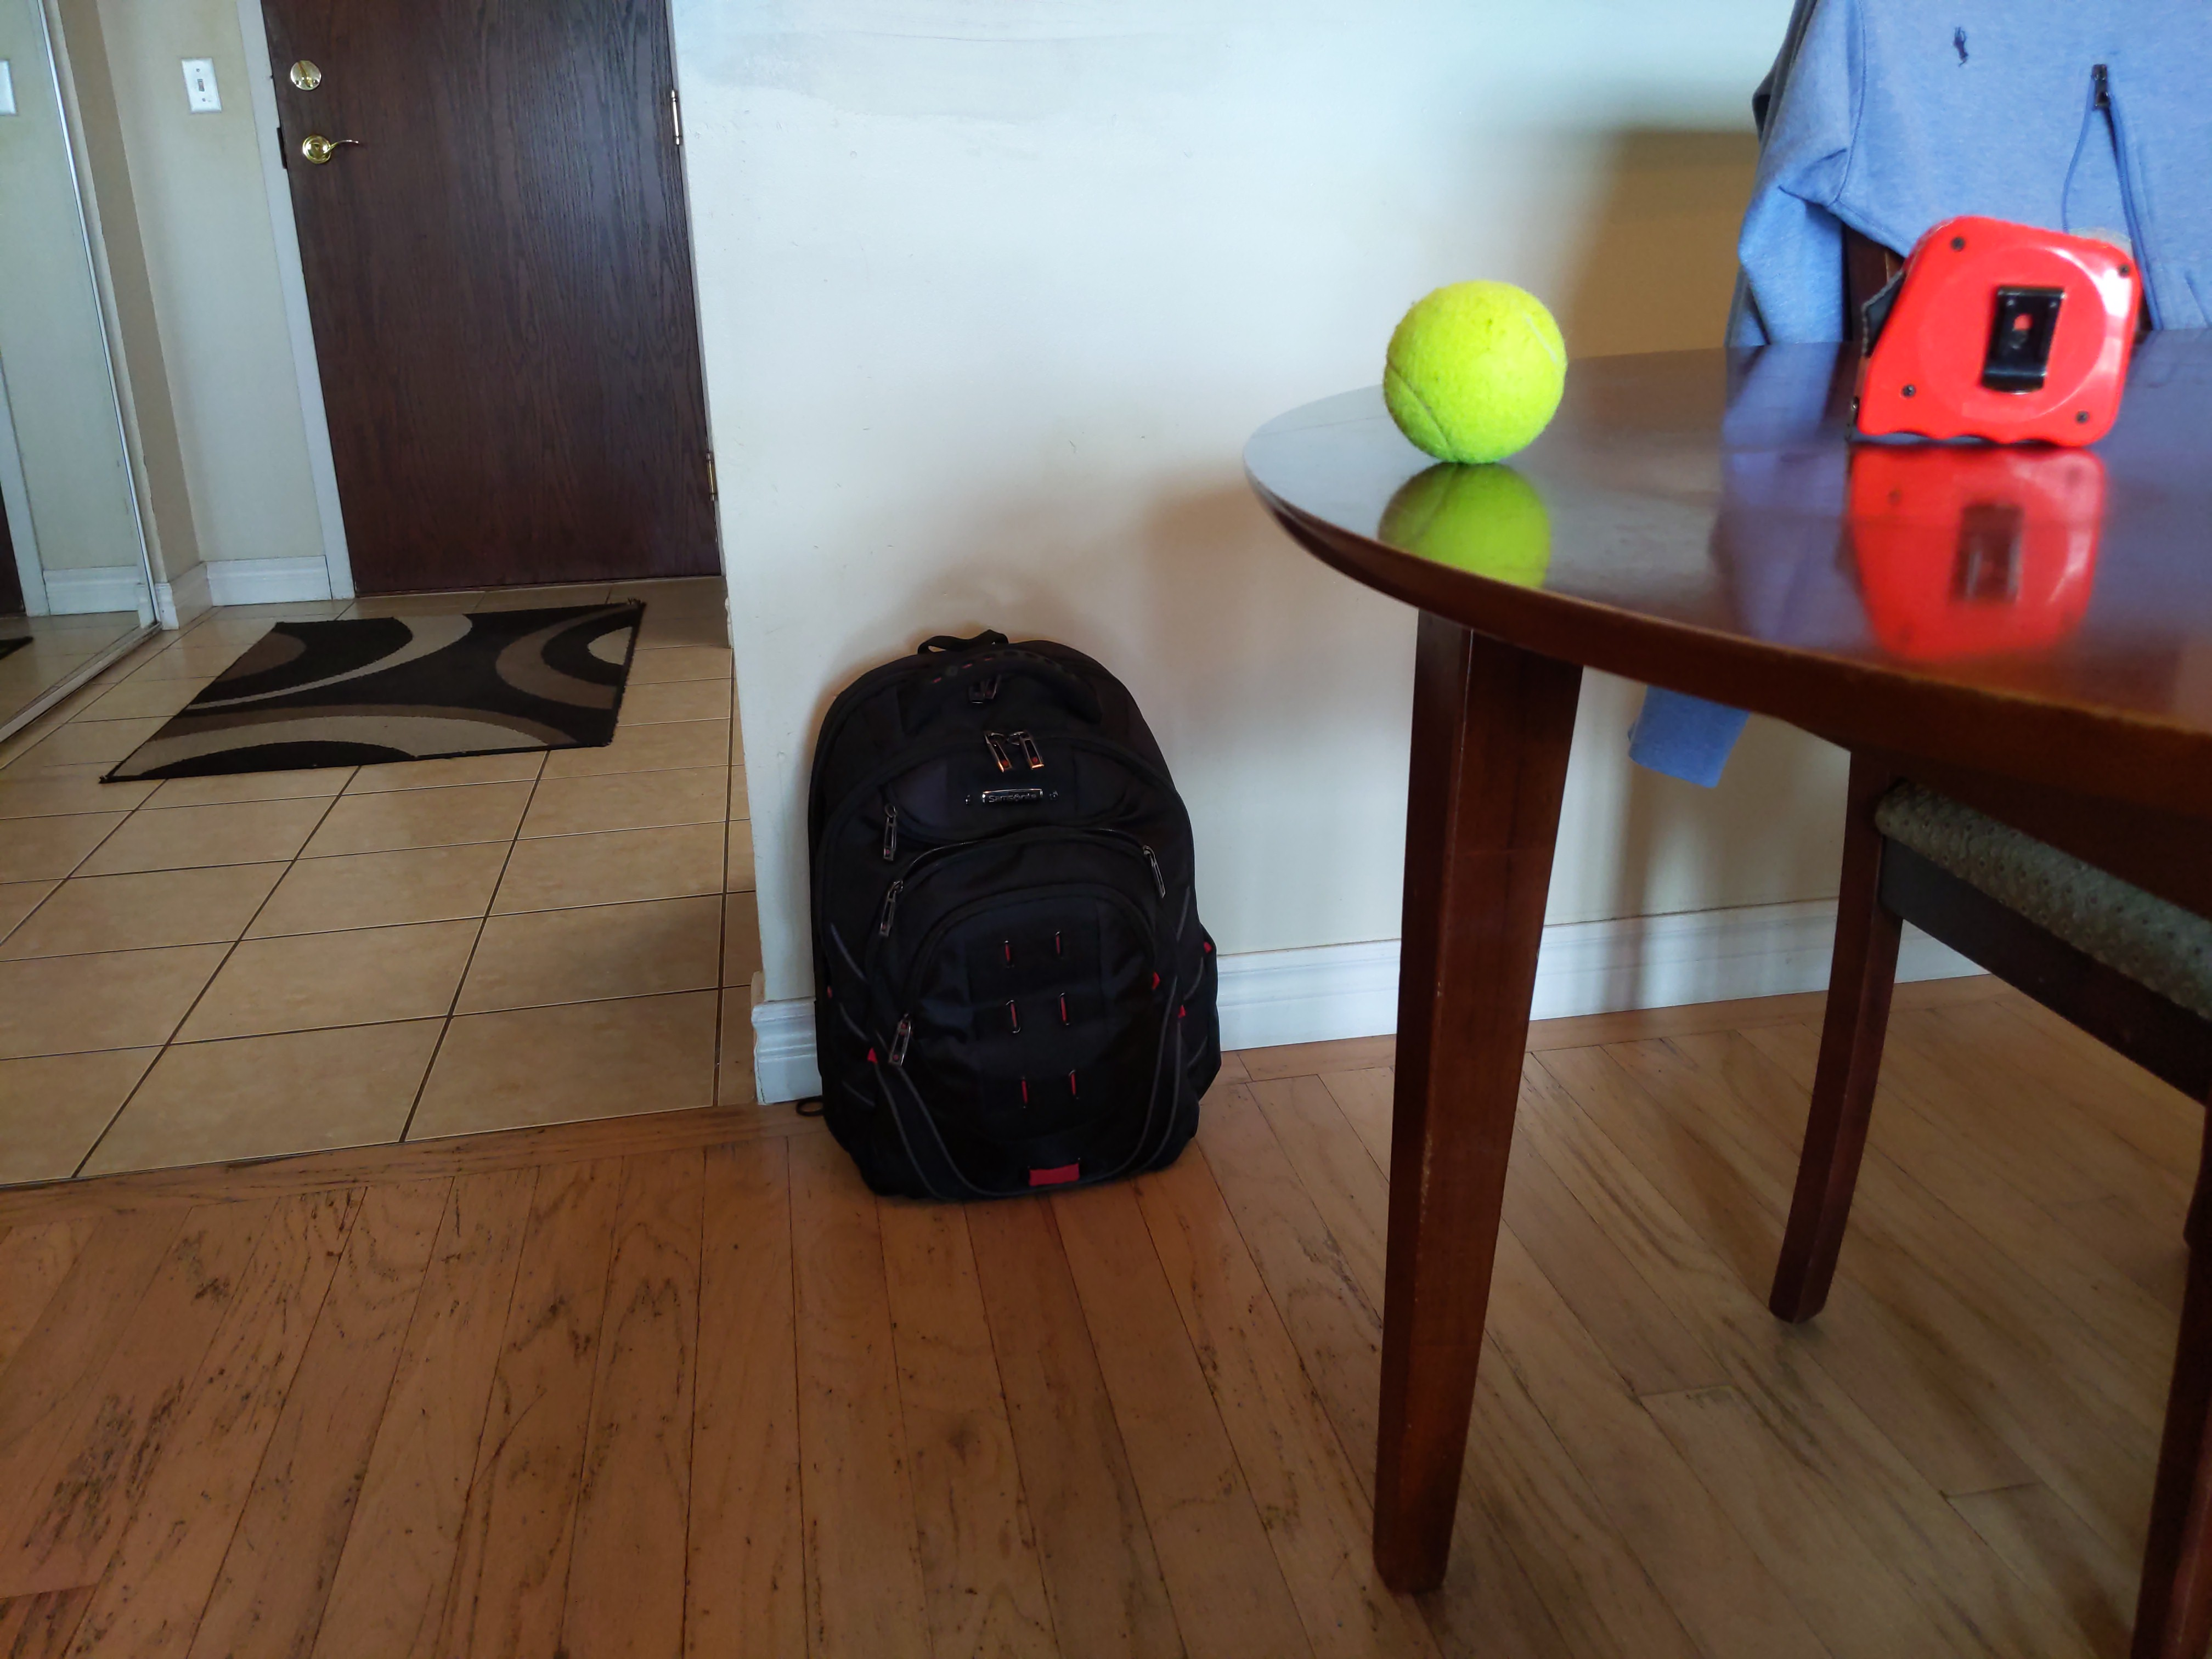
\includegraphics[scale=0.11]{data-collection/apparatus.jpg}
	\caption{Apparatus}
	\label{fig:apparatus}
\end{figure}

\section{Horizontal Motion}

\subsection{Motion Experienced by Object Horizontally}

The object experiences uniform motion horizontally because the velocity remains constant which means that the object is not accelerating. This motion was caused by my hand pushing it in the forwards direction.

\subsection{Calculation of Horizontal Velocity}

\begin{align}
\Delta\vec{d}_x&=\vec{v}_x\Delta{t}\\
38.0\,cm\,[f]&=\vec{v}_x(0.391\,s)\\
\frac{38.0\,cm\,[f]}{0.391\,s}&=\vec{v}_x\\
\vec{v}_x&\approx97.1867\,cm/s\,[f]\\
\Aboxed{\vec{v}_x&\approx0.97\,m/s\,[f]}
\end{align}

$\therefore$ the horizontal velocity of the object is $0.97\,m/s\,[f]$.

\section{Vertical Motion}

\subsection{Motion Experienced by Object Vertically}

The object experiences uniformly accelerated motion vertically because the velocity is changing which means that the object is accelerating, in this case it is speeding up. This motion is caused by the non-contact force of gravity, this is what causes the velocity to change.

\subsection{Calculation of Final Vertical Velocity}

\begin{align}
{\vec{v}_{fy}}^2&={\vec{v}_{iy}}^2+2\vec{a}_y\Delta{\vec{d}_y}\\
{\vec{v}_{fy}}^2&={(0.0\,m/s\,[d])}^2+2(9.8\,m/s^2\,[d])(0.75\,m\,[d])\\
{\vec{v}_{fy}}^2&=(19.6\,m/s^2\,[d])(0.75\,m\,[d])\\
{\vec{v}_{fy}}^2&=14.7\,m^2/s^2\,[d]\\
\vec{v}_{fy}&=\sqrt{14.7\,m^2/s^2\,[d]}\\
\Aboxed{\vec{v}_{fy}&\approx3.8\,m/s\,[d]}
\end{align}

$\therefore$ the final vertical velocity of the object is $3.8\,m/s\,[d]$.

\section{Final Velocity}

\subsection{Calculation of Final Velocity}

The corresponding 2D vector diagram is in the following subsection (see figure \ref{fig:diagram}). The final velocity can be summarized with the following equation:

\begin{align}
\vec{v}_t&=\vec{v}_x+\vec{v}_y\\
\vec{v}_t&=0.972\,m/s\,[f]+3.834\,m/s\,[d]
\end{align}

To solve for the magnitude of the final velocity, we can use the Pythagorean theorem:

\begin{align}
{|\vec{v}_t|}^2&={(0.972\,m/s\,[f])}^2+{(3.834\,m/s\,[d])}^2\\
|\vec{v}_t|&=\sqrt{{(0.972\,m/s\,[f])}^2+{(3.834\,m/s\,[d])}^2}\\
|\vec{v}_t|&\approx3.95529\,m/s\\
\Aboxed{|\vec{v}_t|&\approx4.0\,m/s}
\end{align}

Lastly, to calculate the direction of the final velocity, we can use the tangent inverse function:

\begin{align}
\tan\theta&=\frac{3.834\,m/s\,[d]}{0.972\,m/s\,[f]}\\
\theta&=\tan^{-1}\left(\frac{3.834\,m/s\,[d]}{0.972\,m/s\,[f]}\right)\\
\theta&\approx{75.774}^{\circ}\\
\Aboxed{\theta&\approx{76}^{\circ}}
\end{align}

\begin{align}
\Aboxed{\vec{v}_t&=4.0\,m/s\,[f\,76^{\circ}\,d]}
\end{align}

$\therefore$ the final velocity is $4.0\,m/s\,[f\,76^{\circ}\,d]$.

\subsection{2D Vector Diagram}

\begin{figure}[H]
	\centering
	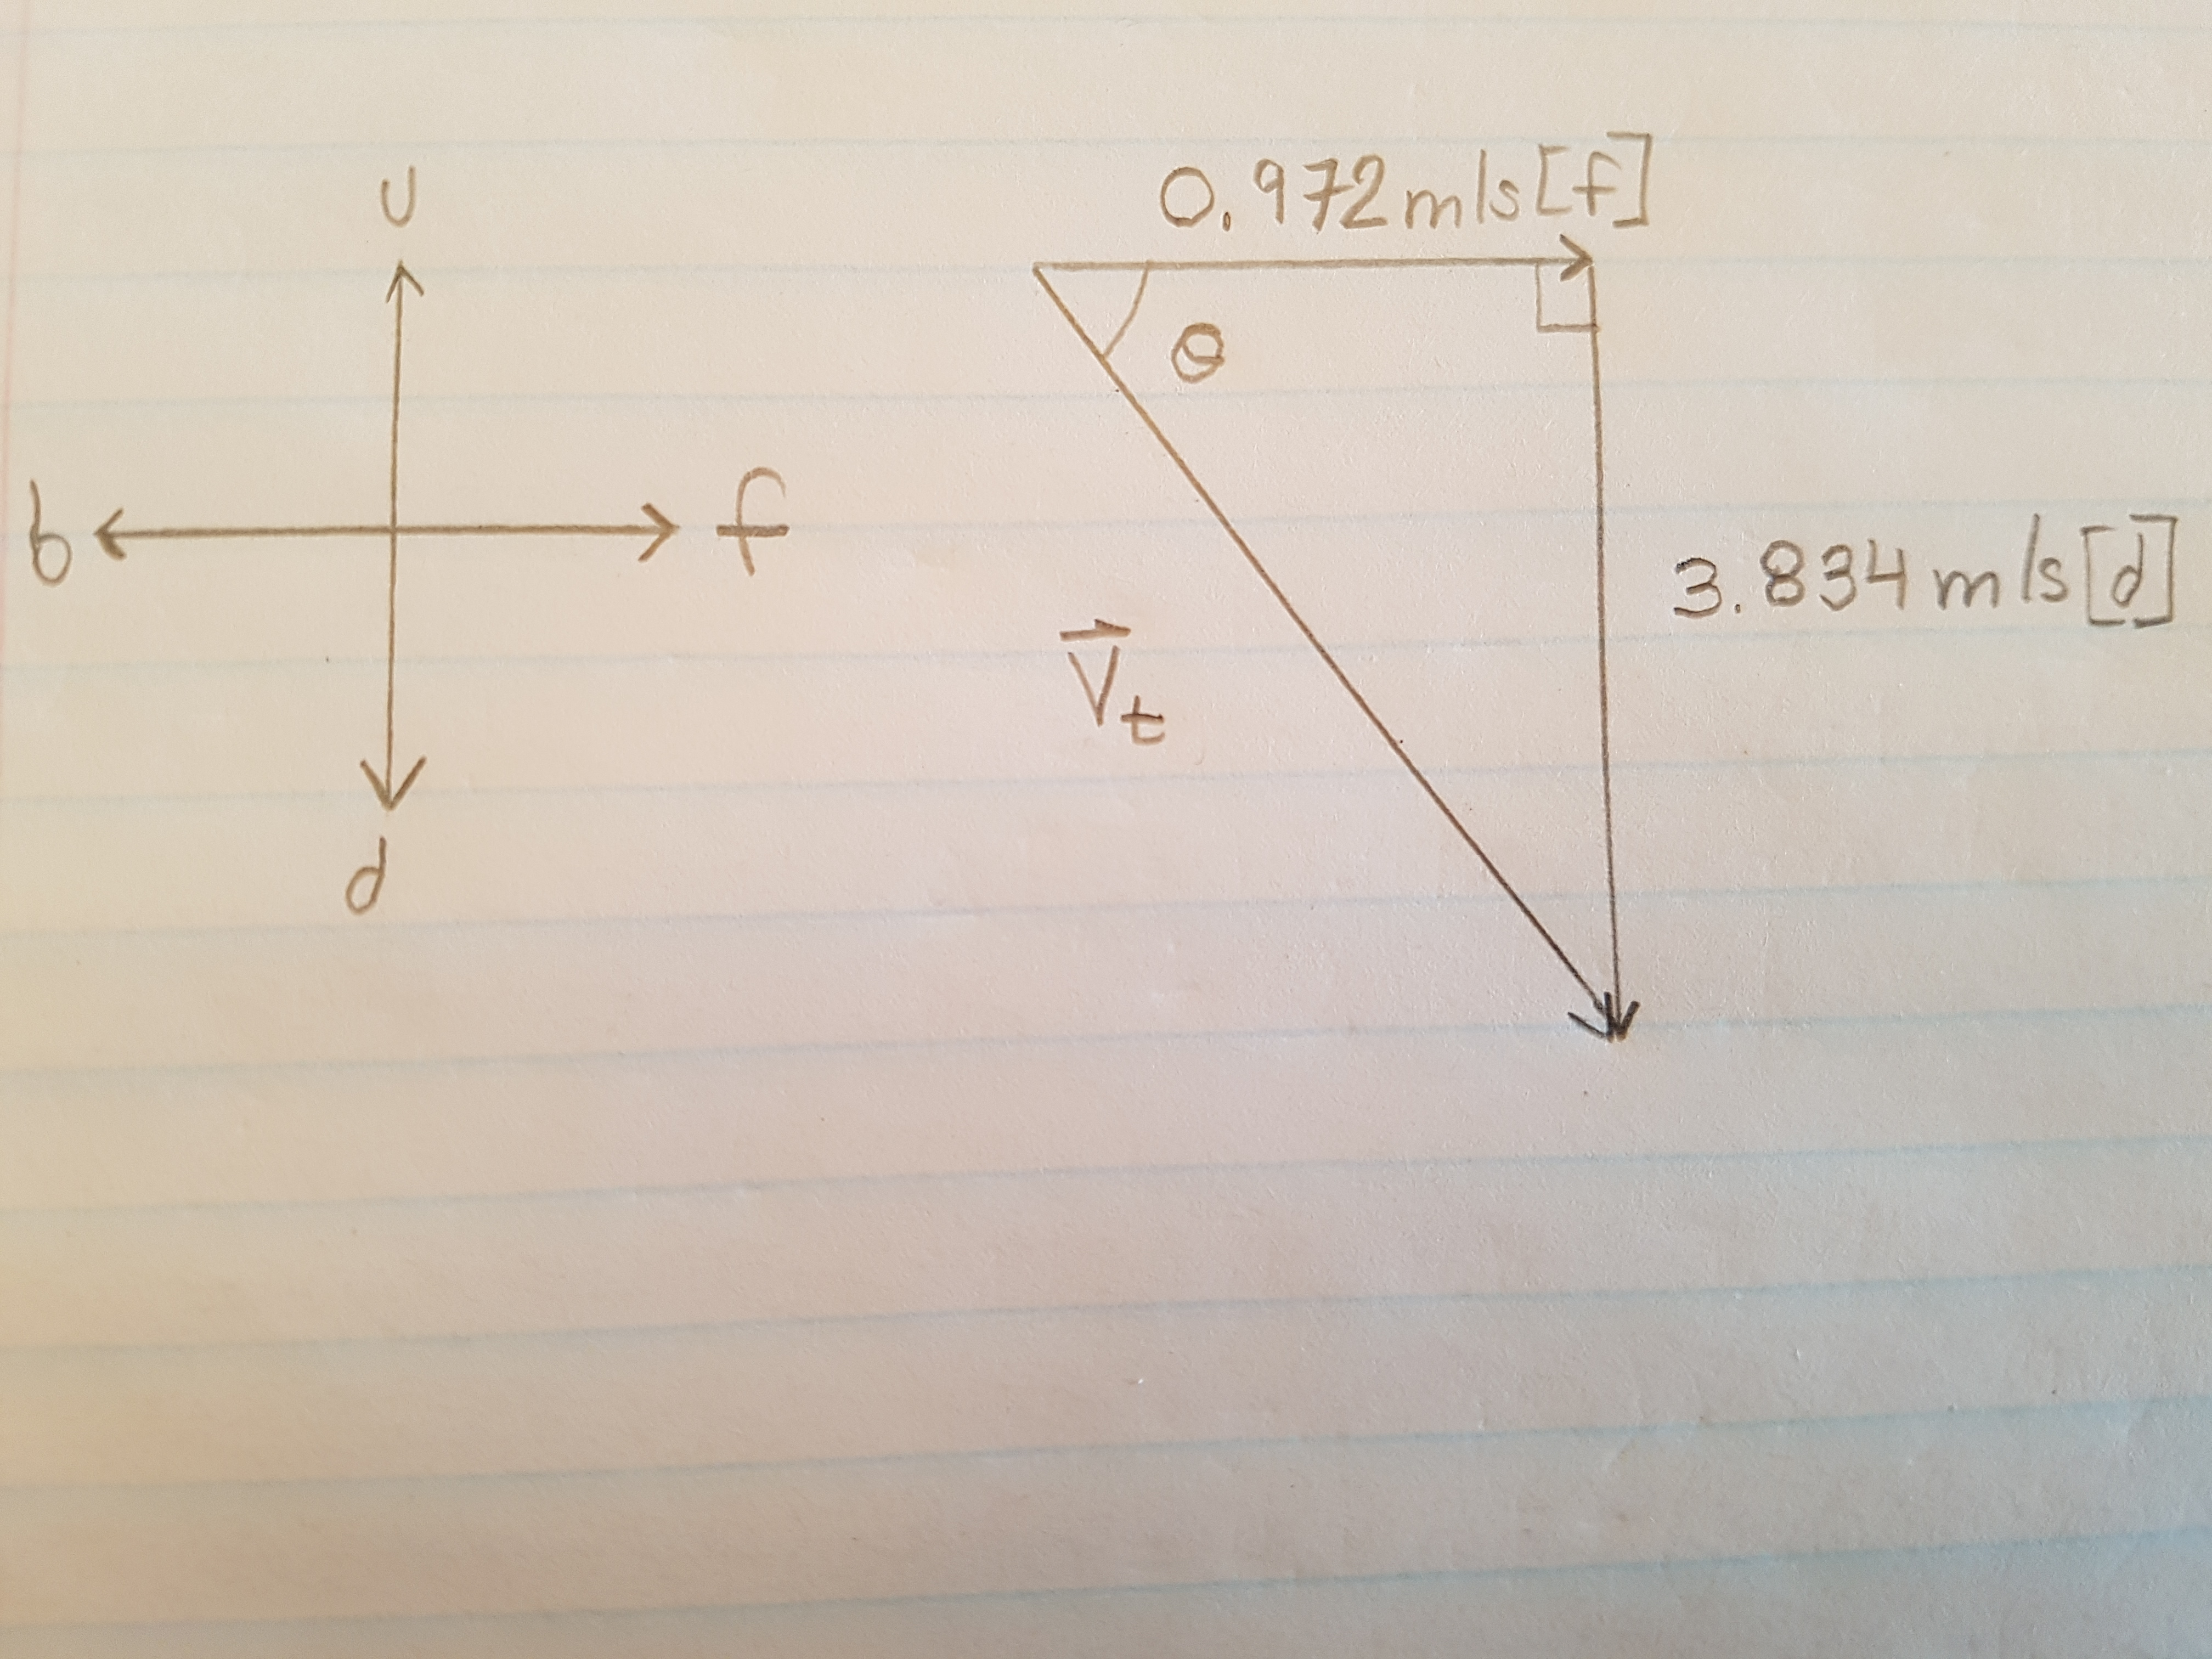
\includegraphics[scale=0.11]{data-collection/2d-vector-diagram.jpg}
	\caption{2D Vector Diagram}
	\label{fig:diagram}
\end{figure}

\end{document}
